\section{Analysis procedure}
This chapter will describe in detail the analysis procedure to select events belonging to the $\gamma (p,n) \pi^+$ channel from the g9a data set corresponding to the linearly polarised beam and longitudinally polarised target settings.
Charged particles are identified with high efficiency in the CLAS detector ($\geq90\%$ \cite{Mecking2003}), so the analysis relies on detecting the $\pi^+$ and reconstructing the neutron from kinematics. The $\pi^+ n$ channel was first identified by filtering the data based on the invariant mass, beta and timing of each $\pi^+$ event. The neutron was then reconstructed using the missing mass technique. Neutral particles could only be detected with a much lower efficiency ($\sim5\%$ for neutrons with momenta $\sim 0.6 GeV/c$ increasing to $\sim 50\%$ for neutrons with momenta $\geq2 GeV/c$  \cite{Mecking2003}), which would significantly reduce the event sample. Once the channel of interest had been identified, the azimuthal ($\phi$) distribution of the $\pi^+$ in the CLAS detector was obtained, binned according to $\pi^+$ centre-of-mass energy, W, and the cosine of the centre-of-mass polar angle, $cos(\theta)$. The data set analysed for this thesis was divided into subsets for each photon beam (or coherent peak) energy setting (730, 930, 1100, 1300, 1500, 1700, 1900,2100 and 2300 MeV) and for each target setting (target polarisation parallel or anti-parallel to the beam), providing in total 18 subsets of data in the energy range 730-2300 MeV (W =1400-2280 MeV). At the binning stage, the data were  also further subdivided according to the specific linear photon beam polarisation setting i.e. whether the electric field vector of the photon beam was parallel to the floor (PARA), perpendicular to the floor (PERP) or unpolarised (AMO). Then I will describe the next stage of analysis, in which the G double-polarisation observable is extracted from the $\pi^+$ azimuthal distributions.

\subsection{Data Reduction}
The BOS files stored on the JLab tape silo contain all the data collected during JLab experiments so that they can be used for a wide range of analyses. Before the analysis of these data could begin a preliminary reduction of the g9a data set was carried out at JLab allowing the reduced files to be copied to the Edinburgh work disks and to also reduce the CPU time required for analysis. The CLAS analysis package, ROOTBEER \cite{rootbeer} was used for the preliminary data reduction process as well as for the subsequent analysis procedure described in this chapter. This is based on ROOT/C++ and interprets the bank structure of CLAS data. In this preliminary event selection two conditions determined the events which were retained:
\begin{enumerate}
\item  For each event, between one and three particles must be detected in conjunction with a hit in the tagger.
\item  Only three combinations of particles were allowed: one positive particle, one positive and one neutral particle, or one positive and two neutral particles. 
\end{enumerate}
The resulting files were then output as more compact ROOTDST (Data Summary Tape) files.

\subsection{The g9a Targets}
In g9a experiment there were three targets simultaneously in the beamline, as shown in Figure \ref{fig:target_draw}.
\begin{figure}[htb]
  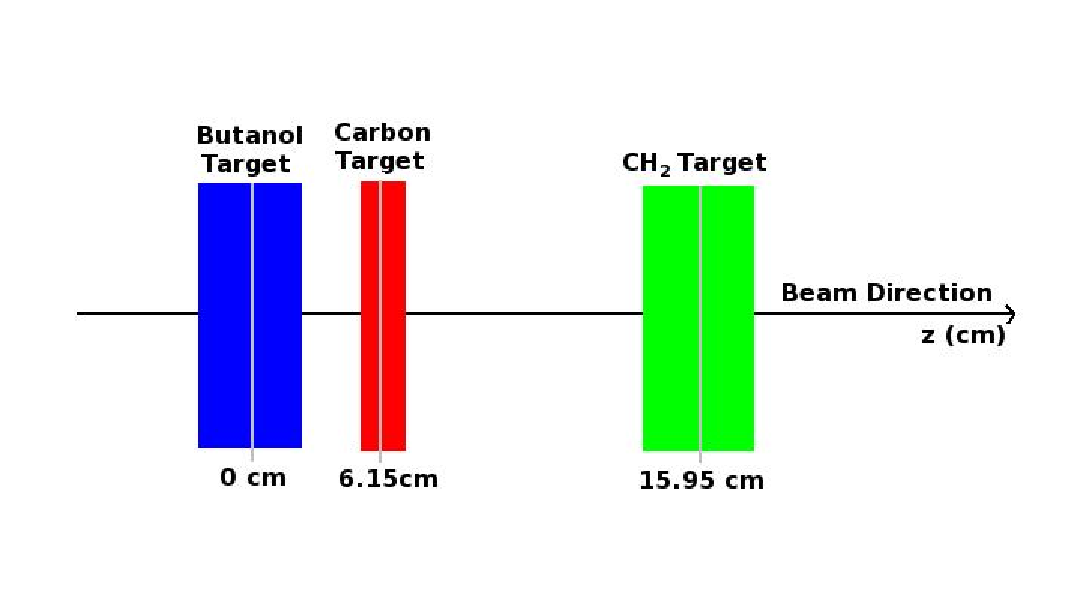
\includegraphics[width=0.8\textwidth]{figures/targets_drawing.png} \\
  \caption{Schematic diagram of the butanol, carbon and $CH_2$ targets in the beamline (not to scale) showing the position of their centres along the z axis. The butanol target was 2.67 mm thick, the carbon target was 1.49 mm thick and the $CH_2$ target was 3.45 mm thick. }
  \label{fig:target_draw}
\end{figure}
The butanol ($C_4 H_9OH$) target formed part of the FROST target system,  providing polarised protons. As butanol contains unpolarised carbon and oxygen atoms as well as polarised hydrogen, analysis of events originating within the carbon target allowed assessment of this unpolarised background contribution. The $CH_2$ target provides unpolarised protons, another useful cross-check for the analysis. Events from each of the three targets were selected by making a cut on the z-vertex position of each event to originate within one of the three targets. The z-vertex position is defined as the point of intersection of the beamline axis with the particle’s trajectory extrapolated back from the drift chambers. Figure \ref{fig:target_pos} shows the z-vertex position of all positive particle events along with the cuts made on the target positions as follows: -2.67 cm $\leq$ z $\leq$ 2.67 cm for the butanol target, 5.0 cm $\leq$ z $\leq$ 7.0 cm for the carbon target and 15.0 cm $\leq$ z $\leq$ 17.0 cm for the $CH_2$ target.
\begin{figure}[htb]
  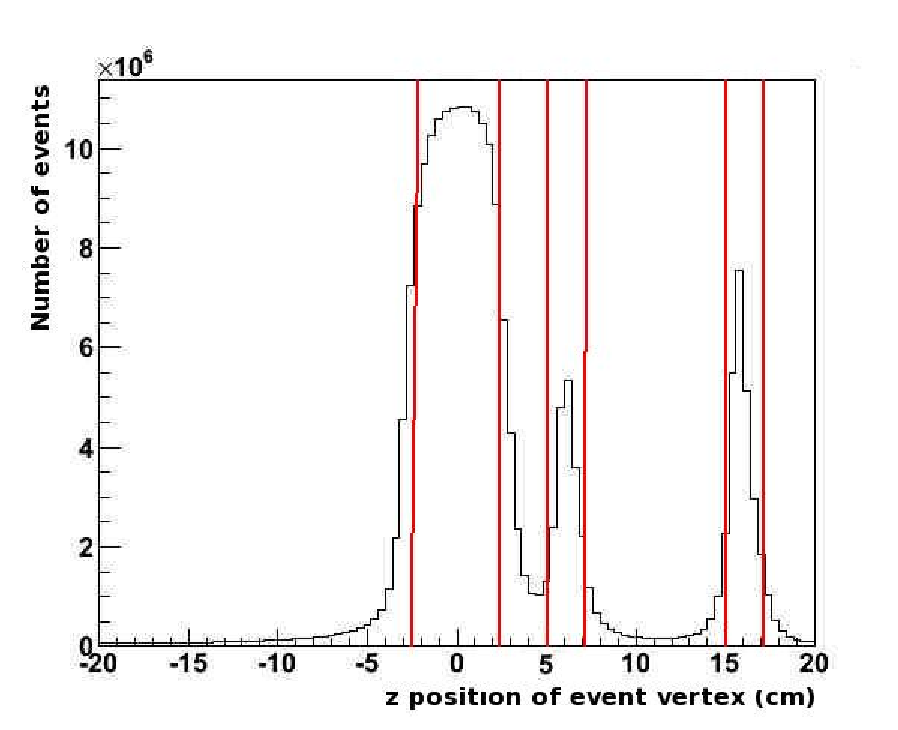
\includegraphics[width=0.8\textwidth]{figures/targets_pos.png} \\
  \caption{Z-vertex distribution of all positively charged particle events. The vertical red lines show the cuts made on the target positions as described in the text.}
  \label{fig:target_pos}
\end{figure}



\subsection{Calculation of the Photon Beam Polarization}
To extract the G observable, as well as the other polarisation observables measured in this experiment, it was necessary to know the degree of linear beam polarisation as accurately as possible. The orientation of the polarisation plane must also be established with accuracy and can be determined from the goniometer settings. The calculation of the degree of linear beam polarisation involves comparing the shape of the coherent Bremsstrahlung spectrum to a spectrum obtained from theoretical Bremsstrahlung calculations. An enhancement plot can be used to separate the coherent contribution from the incoherent contribution to the spectra. The enhancement plots are fit with a theoretical spectrum produced by the Analytical Bremsstrahlung (ANB) Calculation \cite{Natter_2003}\cite{Sabin_2010}. The ANB calculation takes into account 17 experimental parameters characterising the geometry of the radiator, collimator and photon beam. Several of these parameters can be measured experimentally (such as photon beam energy and beam spot size) whereas others (such as electron beam divergence on the radiator) are varied until a good agreement is obtained between the enhancement plot and the ANB calculation. These parameters are then extracted from the fit and are used to calculate the degree of polarisation per event as a function of photon energy. This information is then summarised in lookup tables \cite{Anderson_table}.

\subsection{Cuts}
